\documentclass{article}

\usepackage{neurips_2026}
\usepackage[utf8]{inputenc}
\usepackage[T1]{fontenc}
\usepackage[breaklinks=true]{hyperref}
\usepackage{url}
\usepackage{booktabs}
\usepackage{amsfonts}
\usepackage{amsmath}
\usepackage{nicefrac}
\usepackage{microtype}
\usepackage{xcolor}
\usepackage{graphicx}
\usepackage{subcaption}
\usepackage{float}
\graphicspath{{figures/}}

\renewcommand{\topfraction}{0.95}
\renewcommand{\bottomfraction}{0.90}
\renewcommand{\textfraction}{0.05}
\renewcommand{\floatpagefraction}{0.85}
\setcounter{topnumber}{5}
\setcounter{bottomnumber}{5}
\setcounter{totalnumber}{10}
\setlength{\textfloatsep}{10pt plus 2pt minus 2pt}
\setlength{\floatsep}{8pt plus 2pt minus 2pt}
\setlength{\intextsep}{8pt plus 2pt minus 2pt}

\title{MoleculeLens: Interpretable Drug--Text Retrieval via Salient Molecular Substructures}

\author{%
Anonymous Author\\
Anonymous Institution \\
\texttt{anonymous@anonymous.edu}
}

\begin{document}

\maketitle

\begin{abstract}
Drug--text retrieval systems can connect molecular structures to mechanism descriptions, but most current models are difficult to interpret mechanistically. They often rely on large black-box encoders, and benchmark scores can be inflated by memorized scaffolds, drug names, or target metadata. As a result, it is unclear whether a retrieved match is supported by meaningful molecular substructures or by easier lexical shortcuts. We present \textit{MoleculeLens}, an interpretable drug--text retrieval framework that makes each alignment decision traceable to salient molecular features. MoleculeLens aligns fixed molecular fingerprints and frozen biomedical text embeddings using learned linear projection heads. This deliberately constrained architecture is the core methodological contribution: the molecule-side linear map ranks which ECFP4 substructure bits support a retrieval without rerunning the model for every masked bit. On a scaffold-disjoint ChEMBL benchmark, MoleculeLens improves Recall@1 by 9.6 points and MRR by 4.8 points over MolPrompt, while also exposing when performance depends on drug-name or target/action metadata. Beyond retrieval accuracy, MoleculeLens provides pharmacophore-level explanations for correct matches, faithful diagnostics for failed retrievals, and a same-model analysis of how lexical cues change the molecular features that drive a score. These results show that lightweight linear bridges can make drug--text alignment more interpretable and chemically grounded without giving up competitive top-rank retrieval performance.
\end{abstract}

\section{Introduction}

Drug--text alignment asks whether molecular structures and mechanism descriptions can be embedded in a common space for retrieval~\citep{edwards2021text2mol,liu2023moleculestm,zeng2022kvplm}. The problem is useful for mechanism search, dataset curation, and model validation, but it is hard to trust a high retrieval score by itself: shortcut learning and annotation artifacts can inflate apparent performance~\citep{gururangan2018annotation,geirhos2020shortcut}. Drug names, target labels, and scaffold-correlated train/test examples can make a model look accurate even when the molecular evidence behind a match is weak, motivating scaffold-aware evaluation in molecular learning~\citep{bemis1996frameworks,wu2018moleculenet}. Standard contrastive dual encoders can retrieve well, but their scores give little direct evidence about which substructures support a retrieved mechanism~\citep{radford2021clip,edwards2021text2mol}.

These risks are especially acute in molecule--language retrieval because the text side often contains exact or near-exact identifiers, including drug names, target names, action labels, and curated mechanism templates from resources such as ChEMBL~\citep{gaulton2012chembl,zdrazil2024chembl}. Prior molecule--language systems evaluate retrieval, generation, or representation quality~\citep{edwards2021text2mol,edwards2022molt5,pei2023biot5,liu2023molca,zeng2022kvplm}, but their standard outputs are ranked lists or generated text rather than an explanation path from a retrieval score to the molecular substructures supporting it. Thus, even when leakage controls are reported, the field still lacks a way to ask whether a high-scoring drug--mechanism match is driven by pharmacophoric evidence or by lexical contamination.

The strength of MoleculeLens is a deliberately constrained, computationally efficient design that makes drug--text retrieval interpretable at the ECFP4-substructure level. It freezes the molecule and text encoders, learns only thin linear projection heads, and uses the molecule-side linear map as a lens on ECFP4 substructure bits. The goal is not to build the largest drug--language model. The goal is to make each prediction traceable to chemically meaningful fingerprint environments, so shortcut behavior can be inspected at the substructure level.

\paragraph{Contributions.}
\begin{itemize}
\item \textbf{A linear-bridge retrieval architecture.} MoleculeLens freezes ECFP4 fingerprints and biomedical text embeddings and trains only two linear projection heads, making each drug--text score traceable to ranked fingerprint environments without rerunning the model for every masked bit.
\item \textbf{Strong top-rank retrieval under scaffold shift.} We construct a reproducible ChEMBL benchmark of 2,699 approved-drug mechanism pairs and test on 435 molecules whose Bemis--Murcko scaffolds are unseen during training. On this hard split, MoleculeLens achieves the strongest Recall@1 and MRR among the evaluated cross-modal baselines (R@1 0.225, MRR 0.304), improving Recall@1 by 9.6 points over MolPrompt and 17.0 points over KV-PLM.
\item \textbf{Experimentally validated substructure explanations.} The resulting fast saliency ranking closely matches exact normalized-score gradients (mean Pearson 0.905) and exact leave-one-bit-out score drops (0.947), including failed rank-1 retrievals, showing that the explanations are tied to the learned scoring function rather than illustrative post-hoc overlays.
\item \textbf{Complementary molecule-side and text-side diagnostics.} On the molecule side, MoleculeLens explains correct matches with pharmacophore-level evidence, separates chemically plausible near misses from opaque errors, and exposes lexical leakage: removing only the drug-name span drops Recall@1 by 70.4\% and changes the salient substructures that drive retrieval. On the text side, a contrastive logit lens asks a different question: where in the frozen biomedical text encoder drug-retrievable signal becomes available to the learned bridge.
\end{itemize}

\paragraph{Relation to prior work.}
We separate prior work into systems used as retrieval baselines and systems that motivate the design but target a different use case. The evaluated group in Table~\ref{tab:main-results} includes MoleculeSTM for structure--text retrieval and editing~\citep{liu2023moleculestm}, KV-PLM for biomedical multimodal pretraining~\citep{zeng2022kvplm}, Graphormer as a molecular encoder baseline~\citep{ying2021graphormer}, and MolPrompt as a prompt-based retrieval baseline. These comparisons ask whether MoleculeLens remains competitive under scaffold shift; MoleculeLens differs from them by constraining the alignment to two linear bridges, so each drug--text score can be decomposed into ECFP4 environments.

A broader set of molecule--language and molecular representation models is complementary rather than the main empirical target. Text2Mol motivates natural-language molecule retrieval~\citep{edwards2021text2mol}; MolT5 and BioT5 focus on molecular language modeling and generation~\citep{edwards2022molt5,pei2023biot5}; MolCA studies graph--language alignment~\citep{liu2023molca}; and Uni-Mol, ChemBERTa, and graph pretraining develop stronger molecular representations~\citep{zhou2023unimol,chithrananda2020chemberta,hu2020pretraining}. Adapting these systems to scaffold-disjoint drug--mechanism lookup is a separate modeling problem, whereas MoleculeLens asks what can be gained by pairing fixed ECFP4 fingerprints with a frozen biomedical text encoder and making the resulting scores inspectable. Higher-capacity molecular contrastive systems such as MolCLR, SMICLR, and CLOOME~\citep{wang2022molclr,pinheiro2022smiclr,sanchezfernandez2023cloome} are similarly complementary: they pursue representation quality, while our focus is scaffold-disjoint retrieval with substructure-level mechanistic explanations. The evaluation design follows the molecular-learning practice of scaffold splits~\citep{bemis1996frameworks} and combines it with text leakage controls.

MoleculeLens also builds on the dual-encoder retrieval tradition. Scientific and biomedical text encoders such as SciBERT, PubMedBERT, and S-Biomed-RoBERTa provide frozen language representations for domain text~\citep{beltagy2019scibert,gu2021pubmedbert,deka2021sbiomed}, while CLIP-style contrastive alignment and InfoNCE-style objectives motivate the shared retrieval-space training recipe~\citep{radford2021clip,oord2018infonce}. Related leave-one-out and Hopfield variants show alternative contrastive objectives for small-data alignment~\citep{poole2019variational,furst2022cloob}; MoleculeLens instead uses the linearity of the trained bridge as the route to substructure-level explanation.

The interpretability component is related to sparse and linear feature analysis~\citep{bricken2023monosemanticity,templeton2024monosemanticity} and attribution-graph work~\citep{lindsey2025attribution}, but our features are chemically grounded from the start because ECFP4 bits correspond to circular molecular environments~\citep{rogers2010ecfp} recoverable with RDKit~\citep{rdkit}.

\section{MoleculeLens Framework}
\label{sec:framework}

\paragraph{Architecture.}
Figure~\ref{fig:architecture-main} summarizes the MoleculeLens architecture. MoleculeLens does not attempt to interpret every hidden unit of a large multimodal model. Instead, it inserts a small linear bridge between a fixed molecular representation and a frozen biomedical text encoder. That bridge creates a shared retrieval space and, because the molecule-side map is linear, a direct route from each retrieval score back to ECFP4 substructures.

\begin{figure}[!htbp]
  \centering
  \makebox[\linewidth][c]{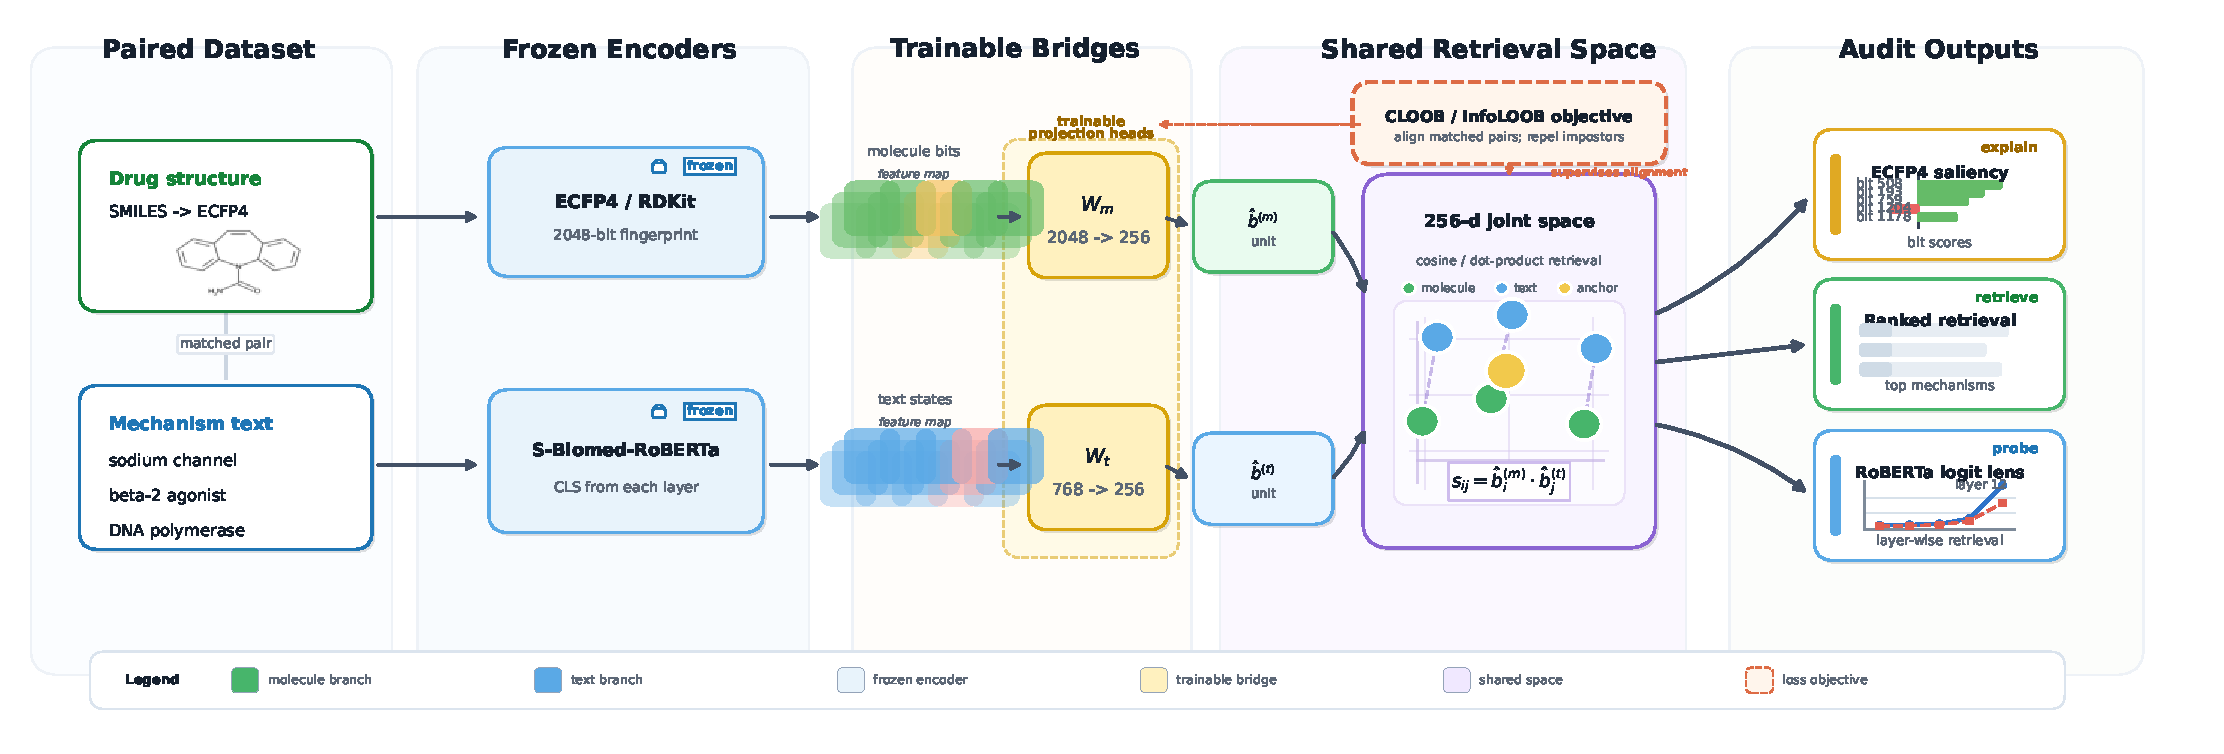
\includegraphics[width=1.02\linewidth]{fig_architecture.pdf}}
  \caption{\textbf{MoleculeLens architecture for interpretable drug--text retrieval.} A fixed RDKit ECFP4 fingerprint and a frozen biomedical text encoder are connected by two learned linear projection heads trained with a symmetric InfoNCE retrieval objective. Because the molecule-side head is linear, each drug--text score can be traced to ranked ECFP4 fingerprint environments without rerunning the model for every masked bit. The same trained text head is reused as a layer-wise logit lens to identify where drug-retrievable information appears in the frozen text encoder.}
  \label{fig:architecture-main}
\end{figure}

\paragraph{Linear bridge retrieval model.}
For drug $i$, RDKit computes $x_i$, a radius-2, 2048-bit ECFP4 fingerprint whose bits encode local molecular environments~\citep{rogers2010ecfp}. For text $i$, a frozen S-Biomed-RoBERTa sentence encoder~\citep{deka2021sbiomed} produces a CLS-style embedding $z_i$. MoleculeLens learns only two linear projection heads,
\begin{equation}
b_i^{(m)} = W_m x_i + b_m,\qquad b_i^{(t)}=W_t z_i+b_t,
\end{equation}
followed by $L_2$ normalization and cosine scoring. Training uses symmetric InfoNCE~\citep{oord2018infonce} with same-target weighting and a hardest-same-target margin term. The scaffold model uses batch size 512, learning rate $10^{-3}$, weight decay $10^{-4}$, temperature 0.07, margin 0.1, and 100 epochs. All encoders are frozen; only $W_m,b_m,W_t,b_t$ are trained. Training the projection heads takes under 30 seconds per run on a single NVIDIA GPU; ECFP4 attribution and contrastive logit-lens analyses each complete in under 10 minutes. The dominant cost is the one-time frozen text encoding shared across experiments. Additional implementation details are in Appendix~\ref{app:architecture}.

\paragraph{Substructure saliency from the molecular bridge.}
The normalized retrieval score is
\begin{equation}
s_{ij}=\hat{b}_i^{(m)}\cdot\hat{b}_j^{(t)}
=\mathrm{normalize}(W_m x_i+b_m)\cdot\mathrm{normalize}(W_t z_j+b_t).
\end{equation}
Because $W_m$ is linear, we use the closed-form ECFP4 saliency proxy
\begin{equation}
\label{eq:attribution}
\mathrm{attr}_k(i,j)=\bigl[W_m^\top\hat{b}_j^{(t)}\bigr]_k,
\end{equation}
where $\hat{b}_j^{(t)}=\mathrm{normalize}(W_tz_j+b_t)$. Equation~\ref{eq:attribution} is a fast ranking proxy rather than an exact causal decomposition: the exact normalized score also depends on the molecule-side bias and $\|W_mx_i+b_m\|$. This is why the experimental section validates it against exact gradients and exact leave-one-bit-out score drops before using it for chemical interpretation.

\paragraph{Diagnostics enabled by the same bridge.}
The same linear bottleneck supports two complementary kinds of diagnostic analysis. The first is molecule-side interpretability: saliency over present ECFP4 bits lets us inspect correct and incorrect retrievals as substructure-level decisions, and removing only the explicit drug-name span at inference tests whether lexical leakage changes which molecular features are salient. The second is text-side localization: applying the trained text bridge to each hidden layer of the frozen text encoder does not explain atoms or fingerprint bits, but instead asks where drug-retrievable text information becomes available to the shared retrieval space.

\section{Experimental Validation}
\label{sec:experiments}

\paragraph{Dataset and setup.}
We construct the benchmark from ChEMBL~\citep{gaulton2012chembl,zdrazil2024chembl} by filtering for approved drugs (\texttt{max\_phase=4}), valid mechanism text, and parseable canonical SMILES. The final dataset contains 2,699 drug--text pairs spanning 1,196 unique Bemis--Murcko scaffolds. The primary \texttt{text\_rich} field concatenates four fields in order: mechanism of action, target name, action type, and drug name.
The main split uses seed 0 over unique scaffolds: 2,019 train examples, 245 validation examples, and 435 held-out test examples whose scaffolds are unseen during training. We report text-query retrieval against a molecule gallery using Recall@1, MRR, Recall@5, and Recall@10 for apples-to-apples comparison with baselines. All main-table rows use single-label diagonal evaluation: a prediction is counted correct only when the exact matching row is returned. This is intentionally conservative for drugs with multiple ChEMBL mechanism rows, but it is the only consistent apples-to-apples protocol for baselines where per-example ranked lists are not available.

Several test drugs appear under multiple target--action rows. For attribution analyses, same-drug and wrong-but-close filtering use RDKit \texttt{FragmentParent} standardisation over SMILES to avoid treating salt or formulation variants as independent structures. In the canonical scaffold test set, 193 of 435 rows belong to 76 parent structures with multiple mechanism rows.

\subsection{Model Performance: Scaffold Retrieval and Leakage Controls}
\label{sec:results}

Table~\ref{tab:main-results} shows the main comparison. MoleculeLens has the strongest scaffold-split Recall@1 and MRR among the evaluated cross-modal baselines, improving Recall@1 over MolPrompt by 9.6 points and over KV-PLM by 17.0 points. MolPrompt has higher Recall@5/10, so the claim is not leaderboard dominance: MoleculeLens is strongest at top-rank retrieval while remaining competitive at broader candidate coverage. Full-gallery rows are included only as context; the Thin Bridges global result is a memorization-heavy reference, not the main scientific comparison.

\begin{table}[!htbp]
\centering
\small
\caption{\textbf{Model performance under scaffold-disjoint retrieval.} All rows use single-label diagonal evaluation, so a query is counted correct only when it retrieves the exact paired molecule row. Full-gallery rows test easier global lookup and are included only as context; scaffold rows test held-out Bemis--Murcko scaffolds and define the main scientific comparison. MoleculeLens achieves the strongest scaffold Recall@1 and MRR, while MolPrompt remains stronger at broader Recall@5/10 coverage.}
\label{tab:main-results}
\begin{tabular}{l l c c c c}
\toprule
Model & Eval set & R@1 & MRR & R@5 & R@10 \\
\midrule
MoleculeSTM (zero-shot) & Full ($N{=}2699$) & 0.089 & 0.171 & 0.243 & 0.337 \\
Thin Bridges (Global) & Full ($N{=}2699$) & 0.747 & 0.849 & 0.985 & 0.997 \\
MolPrompt (Global) & Full ($N{=}2699$) & 0.123 & 0.264 & 0.405 & 0.590 \\
KV-PLM (Global) & Full ($N{=}2699$) & 0.015 & 0.038 & 0.044 & 0.074 \\
Graphormer (zero-shot) & Scaffold ($N{=}435$) & 0.002 & 0.015 & 0.011 & 0.025 \\
\textbf{MoleculeLens} & Scaffold ($N{=}435$) & \textbf{0.225} & \textbf{0.304} & 0.384 & 0.462 \\
MolPrompt & Scaffold ($N{=}435$) & 0.129 & 0.256 & \textbf{0.400} & \textbf{0.531} \\
KV-PLM & Scaffold ($N{=}435$) & 0.055 & 0.121 & 0.172 & 0.251 \\
\bottomrule
\end{tabular}
\vspace{2pt}
\begin{minipage}{0.98\linewidth}
\footnotesize\textit{Note.} Thin Bridges (Global) trains and tests on the full gallery with no scaffold split. It is included only to bound memorization performance and is not comparable to the scaffold rows.
\end{minipage}
\end{table}

\paragraph{Text-field and leakage controls.}
Because \texttt{text\_rich} includes target/action metadata and an explicit drug field, we report three complementary controls in Table~\ref{tab:controls}. Here, ``leakage drop'' refers to a family of diagnostics rather than a single number: the 51.0\% retrained no-drug drop is the fairest model-comparison baseline, the 70.4\% same-model no-name drop is the fixed-weight causal diagnostic, and the 22.9\% multi-seed proxy mean in Figure~\ref{fig:robustness-main} measures scaffold-partition sensitivity rather than canonical leakage. Removing only the drug field and retraining gives R@1~=~0.110, a 51.0\% relative drop. Holding the rich model fixed and removing only \texttt{Drug: X.} at inference gives R@1~=~0.067, a stricter 70.4\% same-model causal diagnostic. Training on mechanism text alone, removing target name, action type, and explicit drug name, gives R@1~=~0.124 and MRR~=~0.226. Thus target/action fields contribute real signal, but mechanism-only retrieval remains nontrivial and close to MolPrompt scaffold R@1.

\begin{table}[!htbp]
\centering
\footnotesize
\begin{minipage}[t]{0.48\linewidth}
\centering
\caption{\textbf{Text-field ablations and leakage controls.} Canonical scaffold split. ML denotes MoleculeLens; \texttt{text\_rich} includes mechanism, target, action, and drug name. The same-model no-name row removes only the explicit drug-name span at inference with weights fixed.}
\label{tab:controls}
\resizebox{\linewidth}{!}{%
\begin{tabular}{l c c c}
\toprule
Condition & R@1 & MRR & R@1 95\% CI \\
\midrule
ML \texttt{text\_rich} & 0.225 & 0.304 & [0.186, 0.267] \\
ML retrained no-drug & 0.110 & -- & [0.083, 0.140] \\
ML same-model no-name & 0.067 & -- & [0.044, 0.092] \\
ML mechanism-only & 0.124 & 0.226 & -- \\
MolPrompt scaffold & 0.129 & 0.256 & [0.101, 0.164] \\
KV-PLM scaffold & 0.055 & 0.121 & [0.037, 0.081] \\
\bottomrule
\end{tabular}
}
\end{minipage}\hfill
\begin{minipage}[t]{0.48\linewidth}
\centering
\caption{\textbf{Full-objective multi-seed scaffold robustness.} Each row retrains MoleculeLens on a different Bemis--Murcko scaffold split using the complete objective. Seeds 0--4 match the proxy robustness analysis; mean and standard deviation show that top-rank performance is not specific to one split.}
\label{tab:full-loss-multiseed}
\resizebox{\linewidth}{!}{%
\begin{tabular}{r r r r r r}
\toprule
Seed & $n_\text{test}$ & R@1 & R@5 & R@10 & MRR \\
\midrule
0 & 403 & 0.221 & 0.335 & 0.424 & 0.291 \\
1 & 261 & 0.295 & 0.479 & 0.533 & 0.381 \\
2 & 224 & 0.259 & 0.375 & 0.442 & 0.328 \\
3 & 221 & 0.407 & 0.561 & 0.629 & 0.484 \\
4 & 395 & 0.203 & 0.342 & 0.451 & 0.284 \\
\midrule
\textbf{Mean} & -- & \textbf{0.277} & \textbf{0.418} & \textbf{0.496} & \textbf{0.354} \\
\textbf{Std} & -- & 0.081 & 0.098 & 0.085 & 0.083 \\
\bottomrule
\end{tabular}
}
\end{minipage}
\end{table}

The non-overlapping Recall@1 intervals for MoleculeLens \texttt{text\_rich} and MolPrompt support the reliability of the top-rank improvement despite the 435-example test set. Table~\ref{tab:full-loss-multiseed} shows that the complete objective is not weaker than the simplified proxy: mean R@1 is $0.277\pm0.081$ and mean MRR is $0.354\pm0.083$. The higher variance is expected because each seed induces a different scaffold-held-out test set, but every full-loss seed remains above KV-PLM scaffold R@1 and four of five exceed MolPrompt scaffold R@1.

\begin{figure}[!htbp]
\centering
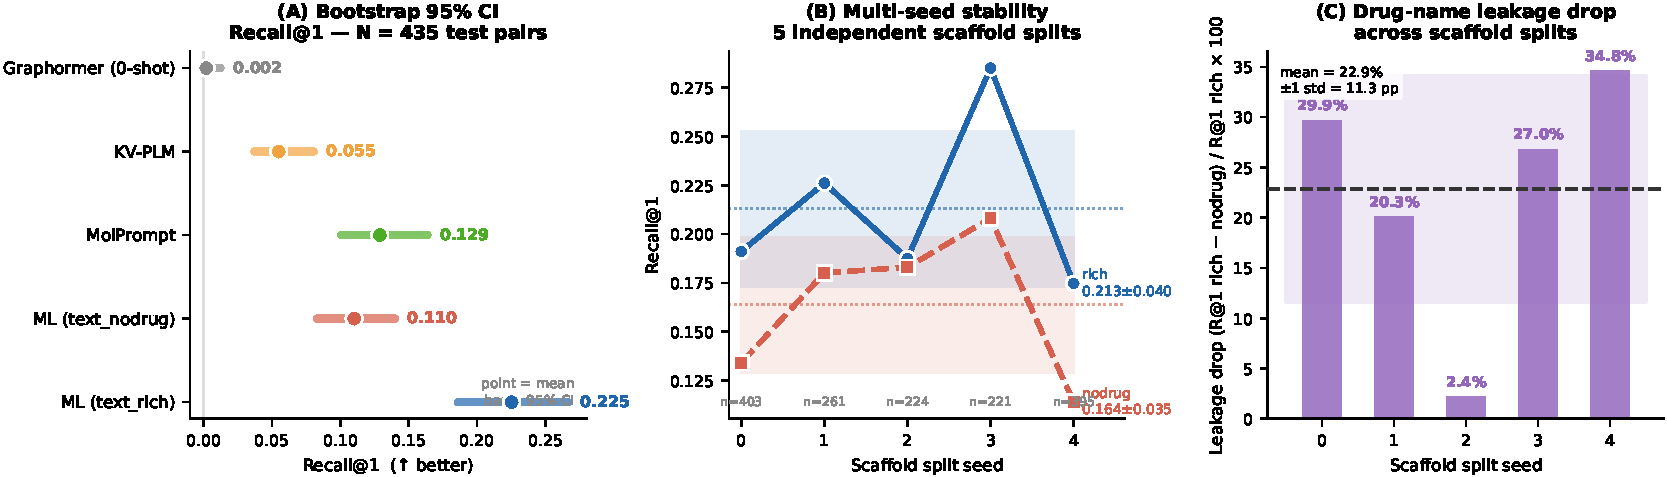
\includegraphics[width=\linewidth]{fig_robustness.pdf}
\caption{\textbf{Robustness of retrieval gains and leakage estimates.} The figure combines bootstrap confidence intervals for canonical scaffold Recall@1, performance variation across five scaffold seeds, and per-seed drug-name leakage drops. Non-overlapping Recall@1 intervals support the reliability of MoleculeLens's top-rank gain over MolPrompt and KV-PLM, while the leakage panel shows that the magnitude of name dependence varies across scaffold partitions.}
\label{fig:robustness-main}
\end{figure}

\subsection{Molecule-Side Interpretability: Attribution Faithfulness and Drug-Specific Substructures}
\label{sec:molecule-side-interpretability}

We validate Equation~\ref{eq:attribution} directly against exact gradients and exact leave-one-present-bit-out score drops over all 435 scaffold test pairs before using it as an interpretability tool.

\begin{table}[!htbp]
\centering
\footnotesize
\setlength{\tabcolsep}{4pt}
\renewcommand{\arraystretch}{0.95}
\caption{\textbf{Faithfulness of the ECFP4 saliency score.} Validation of Equation~\ref{eq:attribution}: all-pair metrics compare fast ECFP4 saliency with exact score-derived references over 435 scaffold test pairs, while stress tests cover failed rank-1 retrievals and distinct drugs sharing identical no-drug text.}
\label{tab:attr-validation}
\begin{tabular}{l c l c}
\toprule
All-pair faithfulness & Value & Stress test & Value \\
\midrule
Pearson(attr, exact gradient) & 0.905 & Incorrect rank-1: Pearson & 0.970 \\
Pearson(attr, exact bit-drop) & 0.947 & Incorrect rank-1: top-10 Jaccard & 0.761 \\
Top-10 Jaccard(attr, exact bit-drop) & 0.710 & Same no-drug text: mean Jaccard & 0.136 \\
 & & Same no-drug text: distinct top-10 sets & 952/954 \\
\bottomrule
\end{tabular}
\end{table}

Table~\ref{tab:attr-validation} supports rank-based use of the saliency proxy. It tracks the exact normalized-score gradient strongly and the exact bit-drop score even more closely. The identical-text test addresses a key conceptual concern: the exact top-10 bit-drop sets are almost never identical across distinct drugs sharing the same no-drug query, so the implemented normalized score is strongly drug-specific. The proxy also remains faithful for failed retrievals, which means incorrect predictions remain interpretable decisions of the learned scoring function rather than cases where the attribution method collapses. Appendix~\ref{app:attribution} provides additional case studies.

\begin{figure}[!htbp]
  \centering
  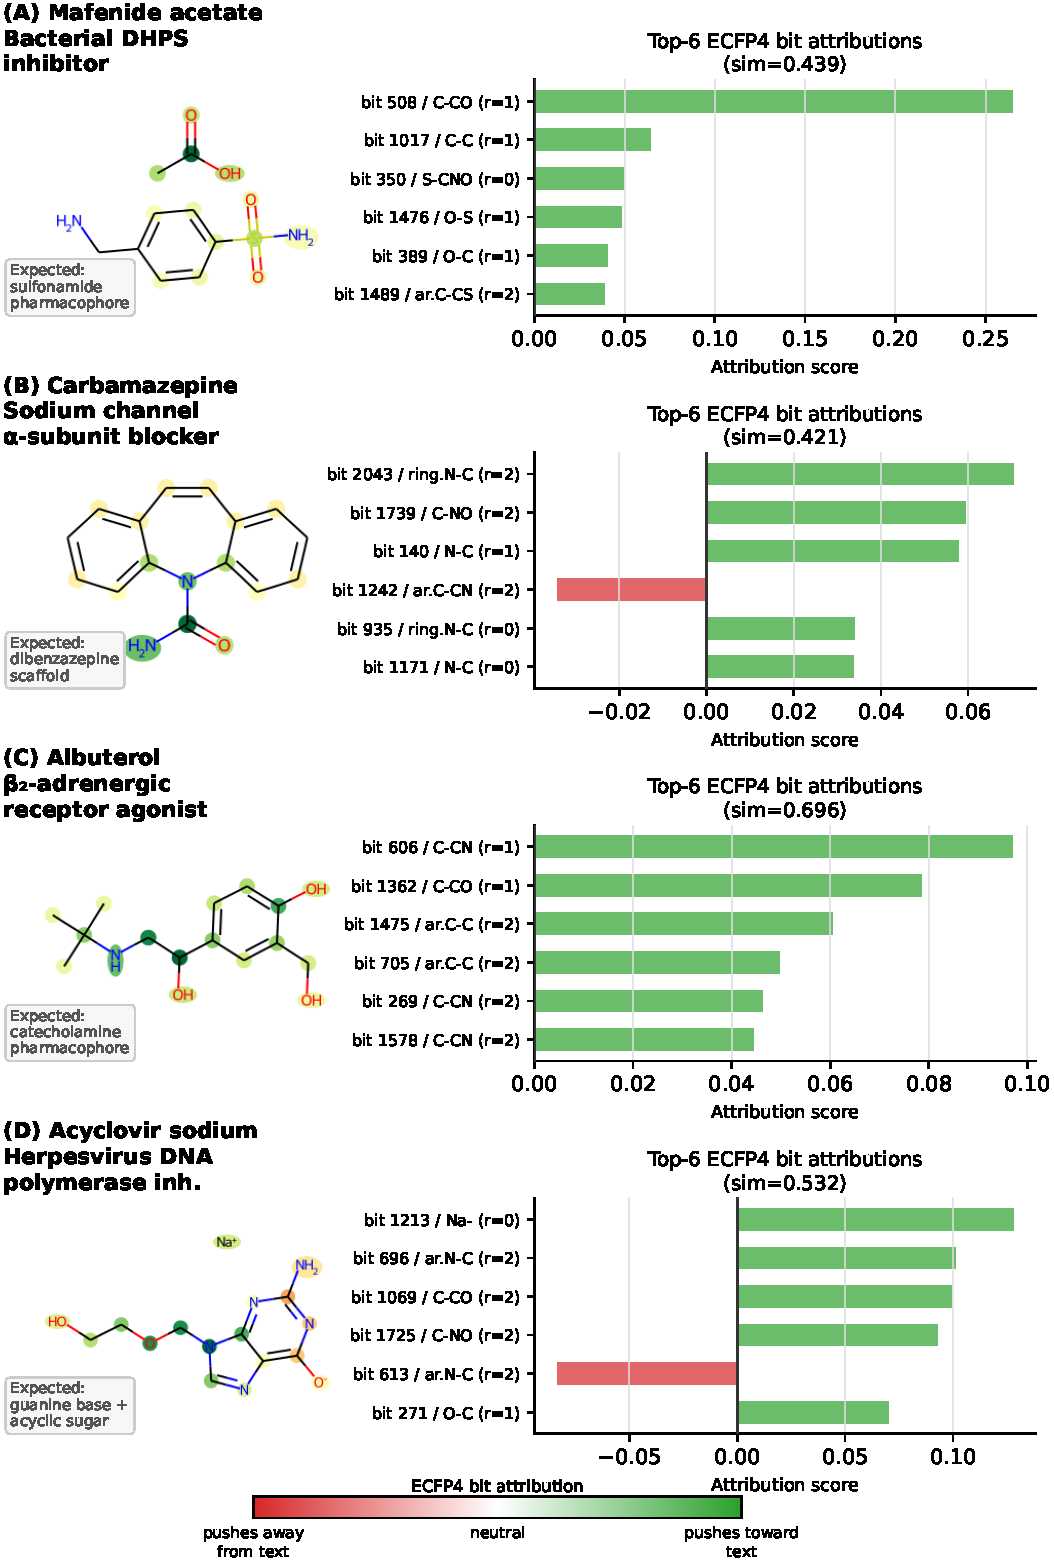
\includegraphics[width=0.96\linewidth]{fig_molecular_lens.pdf}
  \caption{\textbf{Molecular-lens explanations for correctly retrieved mechanisms.} Each panel links a successful drug--text retrieval to the ECFP4 fingerprint environments that most support the score. Atoms are colour-coded by signed attribution value and paired with top-bit bar charts, so the reader can see both where the evidence lies on the molecule and which fingerprint bits drive the ranking. Across the shown examples, high-saliency bits align with pharmacophoric or mechanism-defining regions rather than arbitrary fragments.}
  \label{fig:molecular-lens-main}
\end{figure}

Across these examples and the additional cases in Appendix~\ref{app:attribution}, the highest-saliency fingerprint bits align with known pharmacophoric or mechanism-defining substructures, including steroid cores, sulfonamide groups, nucleoside analogue motifs, beta-lactam rings, and iodinated benzoate rings.

\paragraph{What substructures recur?}
The saliency lens is useful only if it identifies interpretable molecular features rather than a single global shortcut. Appendix Table~\ref{tab:universal-bits} summarizes the most frequent high-saliency ECFP4 bits across the scaffold test set. Bit 1538 is the most common, appearing in the top-10 for 85 pairs; RDKit decoding maps it to a benzene-ring environment with at least one heteroatom substituent at radius 2, a common pharmacophore anchor across several mechanism families. Frequencies drop sharply after the leading bits, and several frequent bits have near-zero mean signed attribution because they appear in both positive and negative contexts. This pattern supports the intended interpretation: MoleculeLens exposes recurring chemically meaningful substructures, but retrieval decisions are not dominated by one universal fingerprint bit.

\paragraph{Explaining near-miss retrievals.}
Faithful attribution is useful beyond correctly retrieved examples. Among rank-2/3 errors after parent-structure filtering, 30 of 43 have attribution correlation above 0.5 between the correct drug and the retrieved drug, with mean correlation 0.569. These are not counted as correct in the diagonal retrieval metric, but the analysis distinguishes chemically plausible near misses from arbitrary failures. Figure~\ref{fig:wrong-close-main} shows a representative case: sodium phenylacetate is ranked second while sodium phenylbutyrate is ranked first, and the two molecules share the same ammonia-lowering mechanism with highly overlapping salient substructures. This does not make the retrieval correct, but it shows that MoleculeLens can expose when an error is driven by related chemical evidence rather than an opaque embedding artifact.

\begin{figure}[!htbp]
  \centering
  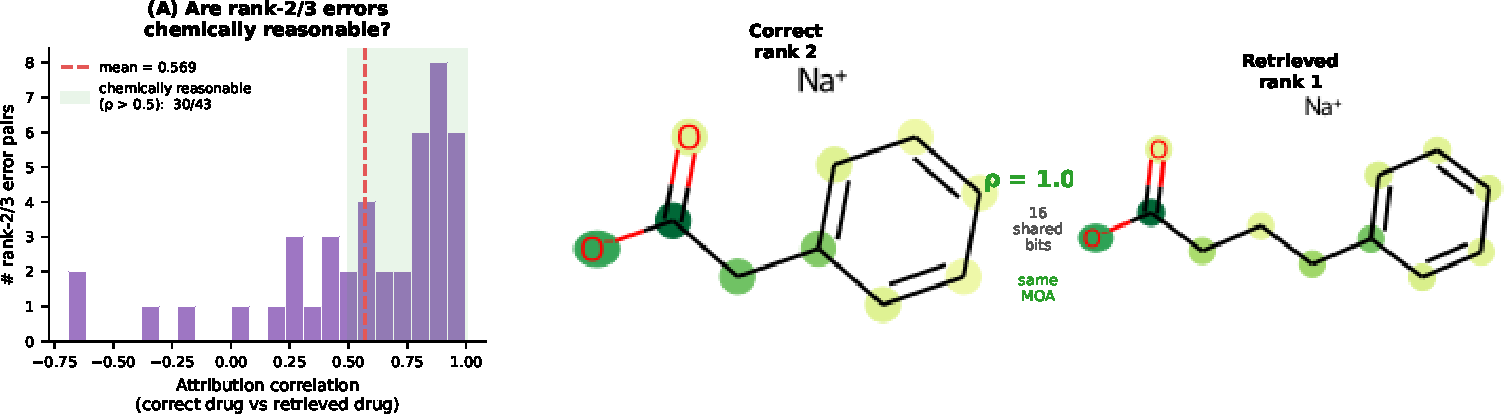
\includegraphics[width=\linewidth]{fig_wrong_close.pdf}
  \caption{\textbf{Near-miss explanations separate chemically plausible errors from opaque failures.} For scaffold-test queries whose correct match is ranked second or third, we compare the saliency vectors of the correct molecule and the top retrieved molecule. High attribution correlation indicates that the model is using overlapping chemical evidence even though the diagonal retrieval metric counts the result as wrong. Sodium phenylacetate retrieved as sodium phenylbutyrate illustrates a high-correlation, same-mechanism confusion.}
  \label{fig:wrong-close-main}
\end{figure}

\paragraph{Same-model leakage attribution.}
We next ask whether the same rich model uses the same substructures when the explicit drug name is removed at inference. For each test pair, let $\mathcal{T}^{\mathrm{rich}}_i$ and $\mathcal{T}^{\mathrm{nodrug}}_i$ be the top-10 saliency-bit sets under the original query and the same query with \texttt{Drug: X.} removed. We compute
\begin{equation}
J_i=\frac{|\mathcal{T}^{\mathrm{rich}}_i\cap\mathcal{T}^{\mathrm{nodrug}}_i|}{|\mathcal{T}^{\mathrm{rich}}_i\cup\mathcal{T}^{\mathrm{nodrug}}_i|}.
\end{equation}
Mean overlap is only $0.356\pm0.161$; 82/435 pairs have $J_i<0.2$, 36/435 have $J_i>0.6$, and 13/435 are leakage candidates that are correct under \texttt{text\_rich}, wrong under the same-model no-name query, and have $J_i<0.2$. This converts the score-level leakage drop into a structural claim: for a substantial subset of test pairs, removing the name changes which molecular features drive retrieval even though model weights are fixed.

\begin{figure}[!htbp]
  \centering
  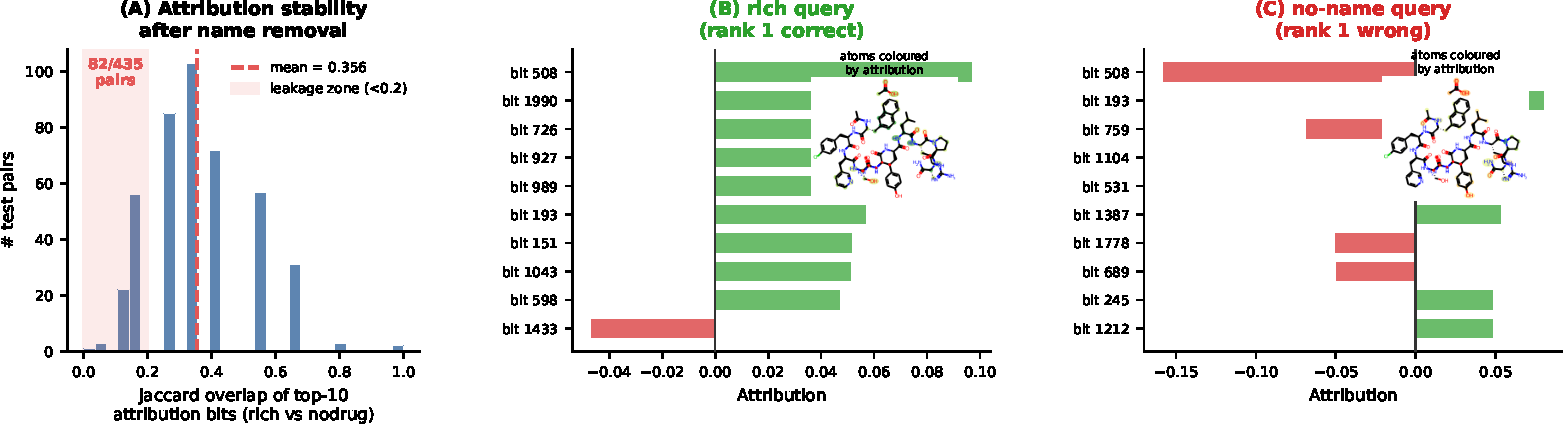
\includegraphics[width=\linewidth]{fig_leakage_substructure.pdf}
  \caption{\textbf{Drug-name leakage changes the substructures used by the same model.} The rich query includes the explicit drug name, while the no-name query removes only that span at inference with all model weights fixed. Low top-10 ECFP4 saliency overlap means that removing lexical information changes which molecular environments drive retrieval. Cetrorelix acetate illustrates a leakage candidate where the prediction and salient substructures both shift after the name is removed.}
  \label{fig:leakage-main}
\end{figure}

\subsection{Text-Side Diagnostic: Where Retrieval Signal Appears}
\label{sec:text-side-diagnostic}

Having established which molecular substructures drive retrieval, we now ask a complementary text-side question: at which layer of the frozen S-Biomed-RoBERTa encoder does drug-retrievable information first become accessible to the learned bridge? This diagnostic does not attribute a retrieval score to atoms or fingerprint bits; it localizes where usable retrieval signal appears inside the frozen text representation.

We adapt the logit-lens idea~\citep{voss2020logitlens} by applying the trained text projection head $W_t$ to the CLS state at each S-Biomed-RoBERTa layer. The diagnostic exactly replays the main rich model at layer 12: the reconstructed embeddings match the saved outputs within $1.21\times10^{-3}$ maximum absolute error and recover R@1~=~0.225. Layers 0--11 are near chance for both rich and retrained no-drug text (R@1 between 0.002 and 0.011), while layer 12 jumps to R@1~=~0.225 for \texttt{text\_rich} and 0.113 for \texttt{text\_nodrug}. This is best viewed as a descriptive sanity check: retrieval signal and the rich-vs-no-name gap both appear in the final contextualized CLS representation, not gradually across intermediate layers. The full layer table and attention visualizations are in Appendix~\ref{app:logit-lens}.

\begin{figure}[!htbp]
  \centering
  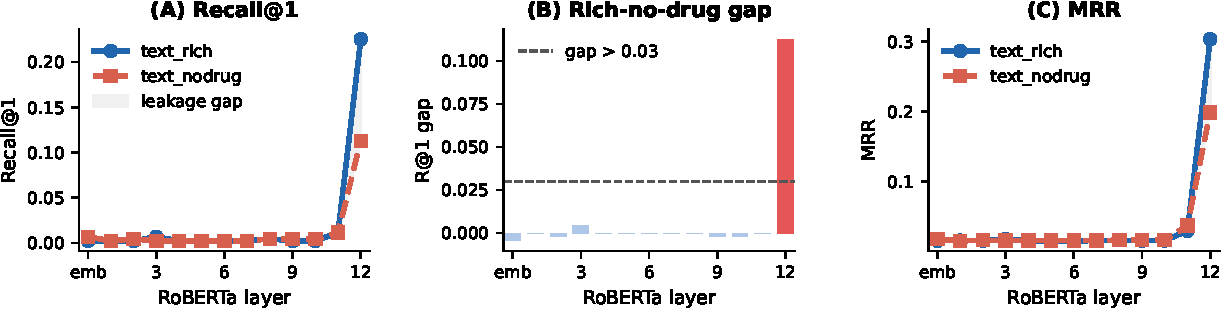
\includegraphics[width=\linewidth]{fig_logit_lens.pdf}
  \caption{\textbf{Text-side logit lens localizes drug-retrievable information to the final RoBERTa layer.} The trained text projection head is applied to CLS embeddings from each frozen S-Biomed-RoBERTa layer and evaluated against the molecule gallery. Retrieval remains near chance through layers 0--11, then layer 12 recovers the main rich-model performance and reveals the gap caused by removing explicit drug names.}
  \label{fig:logit-lens-main}
\end{figure}

\begin{table}[!htbp]
\centering
\footnotesize
\setlength{\tabcolsep}{4pt}
\renewcommand{\arraystretch}{0.95}
\caption{\textbf{Mechanism families with strongest final-layer text retrieval.} Layer-12 Recall@1 under \texttt{text\_rich} on the scaffold test set, sorted by family-level R@1.}
\label{tab:logit-lens-family-main}
\begin{tabular}{l c c l c c}
\toprule
Mechanism family & $n$ & R@1 & Mechanism family & $n$ & R@1 \\
\midrule
Nuclear receptor agonist/antagonist & 18 & 0.611 & Diagnostic agent & 15 & 0.333 \\
Kinase inhibitor & 11 & 0.545 & GPCR agonist/antagonist & 129 & 0.271 \\
Antiviral DNA polymerase inhibitor & 15 & 0.533 & COX inhibitor & 16 & 0.250 \\
Antibacterial & 25 & 0.440 & Ion channel blocker & 41 & 0.195 \\
Other & 165 & 0.152 & & & \\
\bottomrule
\end{tabular}
\end{table}

Layer-12 retrieval is heterogeneous across mechanism families (Table~\ref{tab:logit-lens-family-main}): nuclear-receptor, kinase, antiviral, and antibacterial families show the clearest signal, while GPCR and Other remain harder. This points to curated mechanism text and family-specific lexical structure rather than chemically useful retrieval signal in intermediate RoBERTa layers.

\section{Discussion and Limitations}
\label{sec:discussion}

MoleculeLens is not a claim that frozen ECFP4 plus a linear bridge solves scaffold-generalized drug--text retrieval. Its narrower contribution is that a lightweight model remains competitive at top-rank scaffold retrieval while making its decisions inspectable at the ECFP4-substructure level. The saliency proxy is validated against exact score-derived quantities, remains faithful on retrieval failures, and exposes same-model drug-name leakage as a shift in salient molecular features.

The benchmark has important limitations. The rich text field includes target and action metadata, and the mechanism-only ablation confirms that these fields contribute retrieval signal; the rich-text result should therefore be interpreted as curated mechanism-metadata retrieval rather than pure free-text mechanism understanding. Implicit lexical cues, such as proprietary-name fragments embedded in mechanism text, are not removed by the no-drug ablation and may still inflate no-drug scores. The dataset covers FDA-approved drugs with curated ChEMBL mechanisms and does not establish generalization to investigational compounds or non-ChEMBL prose. Finally, the baseline set does not include adapted MolT5, BioT5, Uni-Mol, MolCA, or chemistry-LLM retrieval systems; these require nontrivial task adaptation and remain important future comparisons.

\paragraph{Reproducibility and intended use.}
The scaffold split, paper-facing tables, and main-number manifests are released to make the benchmark's leakage controls visible rather than implicit. Changing from scaffold-held-out to full-gallery evaluation, or from same-model no-name ablation to retrained no-drug comparison, answers a different scientific question, so we report rich, mechanism-only, and no-name conditions side by side. MoleculeLens is an interpretability tool, not a clinical or regulatory decision system: its use is to show which fingerprint environments support a proposed structure--mechanism match and whether those environments shift under text perturbations.

\paragraph{Future interpretability directions.}
The shared 256-dimensional embedding space is a natural target for sparse autoencoder analysis~\citep{templeton2024monosemanticity,bricken2023monosemanticity} and cross-modal crosscoders~\citep{lindsey2025attribution} that separate genuine structure--mechanism features from text-only leakage. MoleculeLens leaves these extensions to future work, but supplies the fixed split, saved embeddings, and substructure-level saliency targets needed to test them.

\paragraph{Benchmark scope.}
The benchmark covers FDA-approved ChEMBL drugs with parseable SMILES and curated mechanism text; it does not cover investigational compounds, unapproved natural products, or out-of-domain mechanism prose. Same-modality text lookup controls access gallery text rather than molecular structure, so we treat them as text-identifiability diagnostics rather than competing molecular-retrieval baselines.

\section{Conclusion}

On a 2,699-pair ChEMBL benchmark with scaffold-disjoint evaluation, MoleculeLens outperforms MolPrompt and KV-PLM on Recall@1 and MRR. MoleculeLens contributes a validated ECFP4 saliency lens that explains correct matches and diagnoses failed retrievals. Its same-model substructure-shift audit under drug-name ablation is a reusable leakage diagnostic for linear dual encoders, testing whether lexical cues change which molecular features drive a score.


{\setlength{\bibsep}{3pt}
\bibliographystyle{plainnat}
\bibliography{refs}
}

\appendix

\section{Additional Benchmark and Evaluation Details}
\label{app:benchmark}

The primary retrieval direction is text query to molecule gallery because this is the direction used by the attribution and logit-lens analyses. The diagonal evaluation protocol and parent-structure handling are summarized in the main text.

\section{Architecture and Implementation Details}
\label{app:architecture}

The model hyperparameters, runtime, and architecture diagram are summarized in the main text.

\section{Robustness Details}
\label{app:robustness}

\begin{table}[!htbp]
\centering
\small
\caption{\textbf{Proxy-objective scaffold variance and leakage sensitivity across seeds.} Five independent Bemis--Murcko scaffold splits are evaluated with the simplified MoleculeLens proxy objective; only the linear projection heads are retrained for each seed. The table reports retrieval metrics and the relative drug-name leakage drop, $(R@1_\text{rich}-R@1_\text{nodrug})/R@1_\text{rich}$, showing that both performance and leakage depend on the held-out scaffold partition.}
\label{tab:multiseed}
\begin{tabular}{r r r r r r r}
\toprule
Seed & $n_\text{test}$ & R@1 & R@5 & R@10 & MRR & Leakage drop \\
\midrule
0 & 403 & 0.191 & 0.377 & 0.459 & 0.287 & 29.9\% \\
1 & 261 & 0.226 & 0.479 & 0.544 & 0.342 & 20.3\% \\
2 & 224 & 0.188 & 0.393 & 0.496 & 0.296 &  2.4\% \\
3 & 221 & 0.285 & 0.525 & 0.634 & 0.402 & 27.0\% \\
4 & 395 & 0.175 & 0.352 & 0.446 & 0.269 & 34.8\% \\
\midrule
\textbf{Mean} & -- & \textbf{0.213} & \textbf{0.425} & \textbf{0.516} & \textbf{0.319} & \textbf{22.9\%} \\
\textbf{Std}  & -- & 0.045 & 0.070 & 0.073 & 0.053 & 12.6\% \\
\bottomrule
\end{tabular}
\end{table}

The corresponding full-loss five-seed check is reported in the main text in Table~\ref{tab:full-loss-multiseed}; the robustness summary figure is shown in Figure~\ref{fig:robustness-main}.

\section{Additional Attribution Analyses}
\label{app:attribution}

For each test pair, we compute Equation~\ref{eq:attribution}, restrict to ECFP4 bits present in the molecule, rank bits by absolute saliency, and decode top-ranked bits with RDKit. Among eight correctly retrieved examples spanning antibacterial, antiviral, nuclear-receptor, opioid, sulfonamide, and diagnostic-agent mechanisms, the highest-saliency bits correspond to pharmacophoric or mechanism-defining regions such as steroid cores, sulfonamide groups, nucleoside analogue motifs, beta-lactam rings, and iodinated benzoate rings.

Figure~\ref{fig:molecular-lens-main} shows representative correct retrievals. Aggregate high-saliency bit frequencies are reported in Table~\ref{tab:universal-bits}.

\begin{table}[!htbp]
\centering
\small
\caption{\textbf{Recurring high-saliency ECFP4 environments across the scaffold test set.} Frequency counts how often each bit appears in the top-10 saliency ranking over 435 test pairs, and mean attribution reports its average signed contribution when present. The leading bits recur across multiple mechanism families, but their signed effects are not uniformly positive, supporting the claim that MoleculeLens exposes recurring chemical motifs rather than one universal shortcut bit.}
\label{tab:universal-bits}
\begin{tabular}{c c c}
\toprule
Bit index & Frequency & Mean attribution \\
\midrule
1538 & 85 (19.5\%) & 0.228 \\
1380 & 74 (17.0\%) & 0.004 \\
1873 & 55 (12.6\%) & 0.000 \\
807  & 44 (10.1\%) & 0.002 \\
715  & 36 ( 8.3\%) & 0.029 \\
350  & 35 ( 8.0\%) & 0.021 \\
1171 & 33 ( 7.6\%) & 0.009 \\
1917 & 32 ( 7.4\%) & 0.001 \\
1039 & 31 ( 7.1\%) & 0.011 \\
80   & 30 ( 6.9\%) & 0.000 \\
\bottomrule
\end{tabular}
\end{table}

The same-model drug-name ablation figure is shown in Figure~\ref{fig:leakage-main}.

\section{Contrastive Logit-Lens Details}
\label{app:logit-lens}

\begin{table}[!htbp]
\centering
\small
\caption{\textbf{Layer-wise text retrieval under rich and no-drug queries.} The trained text projection head is applied to CLS states from selected frozen RoBERTa layers and evaluated against the molecule gallery. Layers 0--11 carry essentially no drug-retrievable signal under either text condition; meaningful retrieval appears only at layer 12, where the rich-vs-no-drug Recall@1 gap becomes visible.}
\label{tab:logit-lens}
\begin{tabular}{c c c c c c}
\toprule
Layer & \multicolumn{2}{c}{text\_rich} & \multicolumn{2}{c}{text\_nodrug} & Gap \\
\cmidrule(lr){2-3}\cmidrule(lr){4-5}
 & R@1 & MRR & R@1 & MRR & R@1 \\
\midrule
0 & 0.002 & 0.016 & 0.007 & 0.018 & --0.005 \\
3 & 0.007 & 0.018 & 0.002 & 0.016 & 0.005 \\
6 & 0.002 & 0.016 & 0.002 & 0.016 & 0.000 \\
9 & 0.002 & 0.016 & 0.005 & 0.017 & --0.002 \\
11 & 0.011 & 0.030 & 0.011 & 0.037 & 0.000 \\
12 & \textbf{0.225} & \textbf{0.304} & \textbf{0.113} & \textbf{0.199} & \textbf{0.113} \\
\bottomrule
\end{tabular}
\end{table}

Mechanism-family Recall@1 is reported in the main text in Table~\ref{tab:logit-lens-family-main}.

\begin{figure}[!htbp]
  \centering
  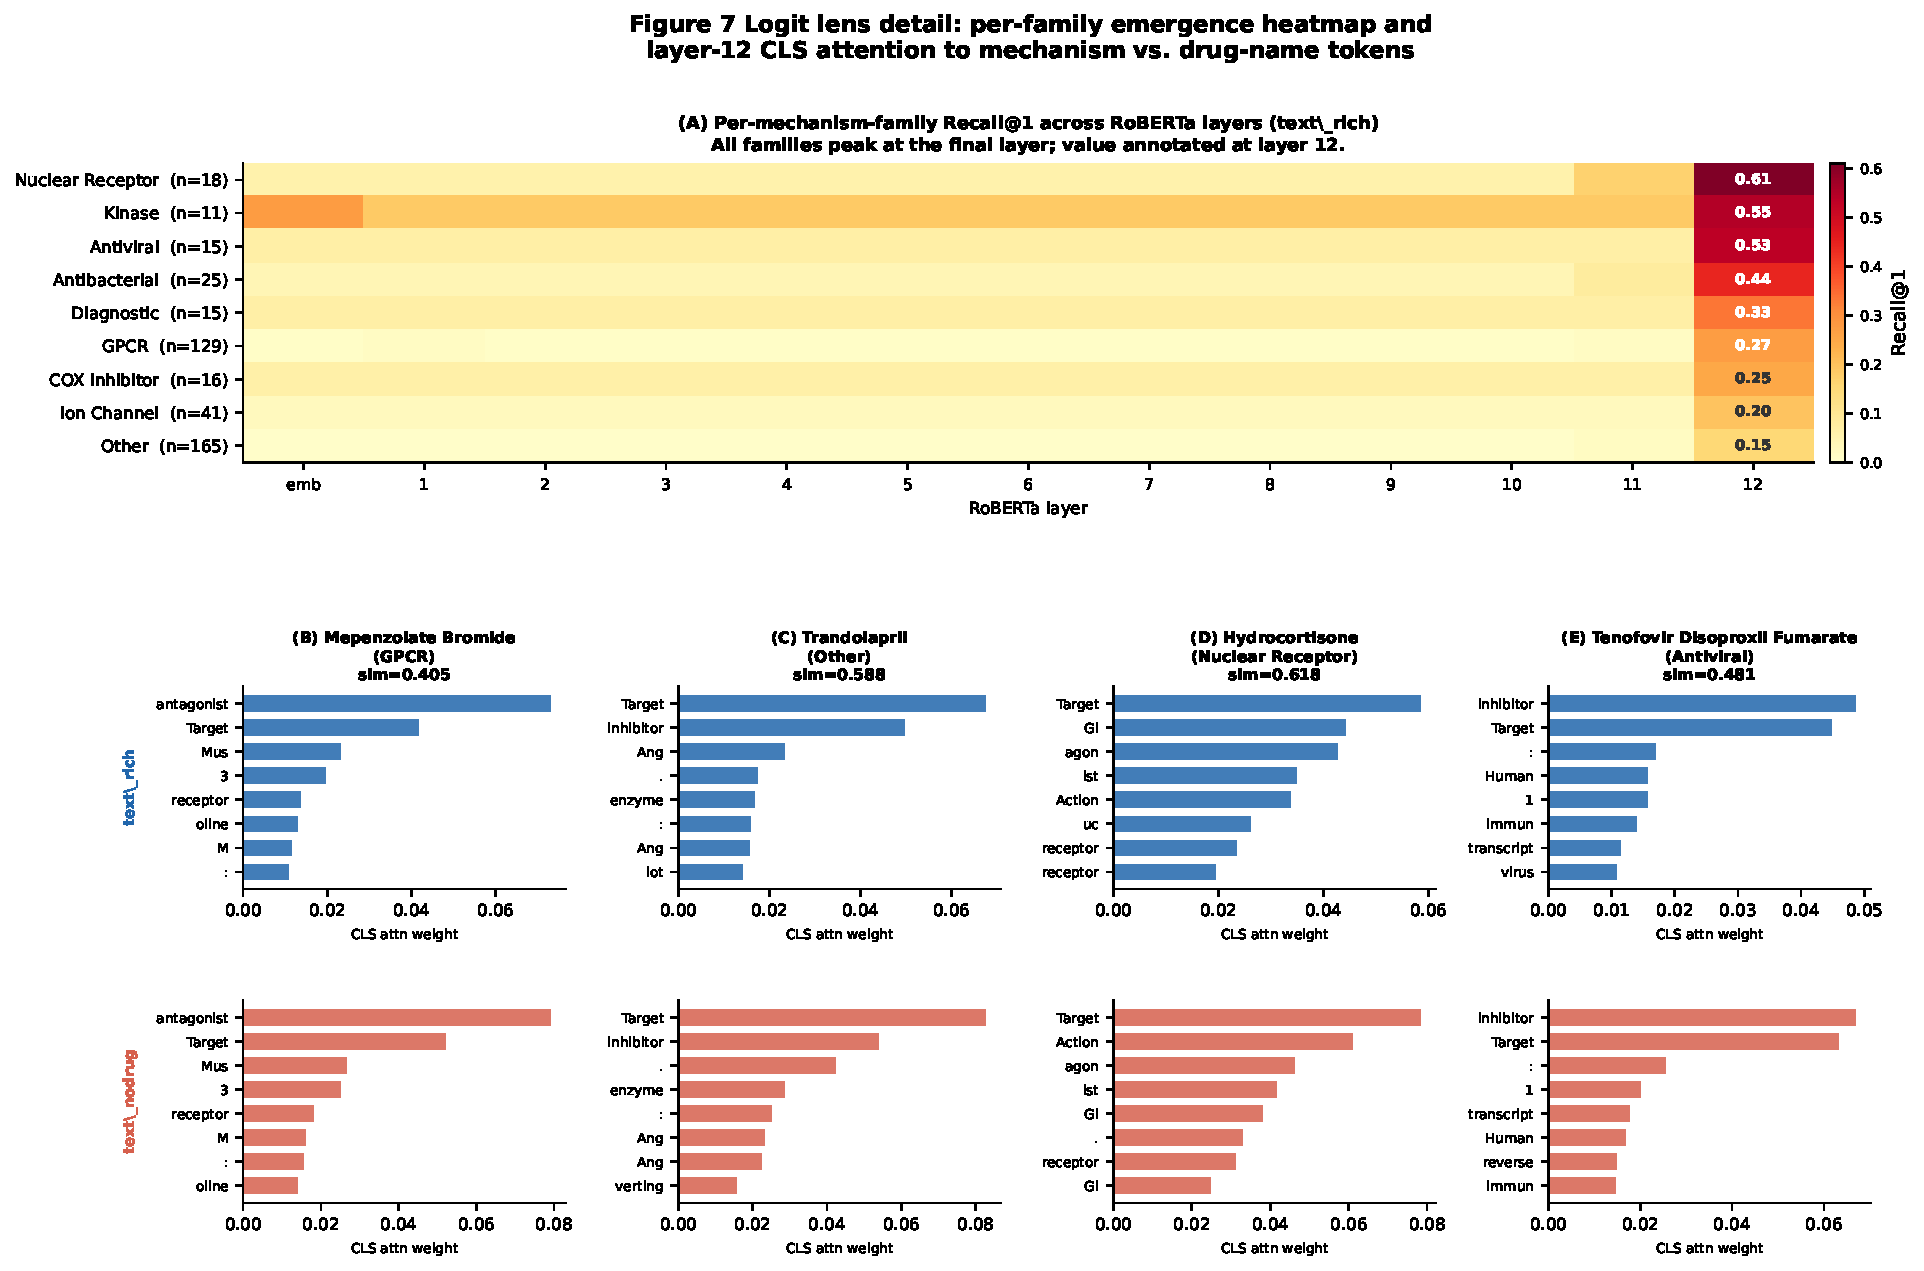
\includegraphics[width=\linewidth]{fig_logit_lens_detail.pdf}
  \caption{\textbf{Detailed text-side diagnostic by mechanism family and attention pattern.} The figure expands the main logit-lens result by showing layer-12 retrieval by mechanism family together with representative CLS attention maps under rich and no-drug text. These panels help distinguish a final-layer retrieval signal from a gradual accumulation of drug-retrievable information across intermediate layers.}
  \label{fig:logit-lens-detail}
\end{figure}

\section{Broader Impacts}

Broader impacts and intended-use considerations are discussed in the main text. In brief, MoleculeLens is an interpretability framework for publicly available ChEMBL drug--mechanism retrieval and is not intended for clinical or regulatory deployment without expert oversight.

\input{checklist}

\end{document}
